\subsection{Connections}\label{sec:mit-connections}
As mentioned in \vref{sec:mit-address} each address comes with a protocol where the protocol represents a connection as presented in \vref{fig:mit-protocol-map}.

\begin{figure}
\centering
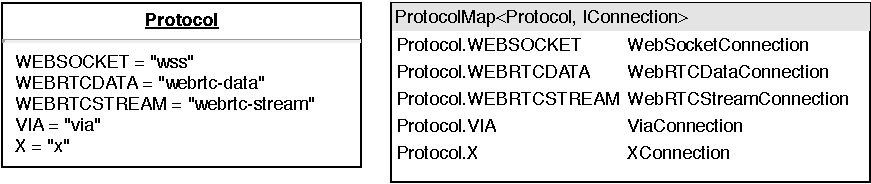
\includegraphics[width=0.75\textwidth]{graphics/implementation/mitosis-architecture-connections-protocol-map.pdf}
\caption{Protocol Map}
\label{fig:mit-protocol-map}
\end{figure}

By extending the \lstinline|ProtocolMap| other connections can be supported. For example when in a future release Bluetooth shall be supported, a new entry can be added in the \lstinline|Protocol| and mapped with the actual implementation in the ProtocolMap.

\begin{figure}
\centering
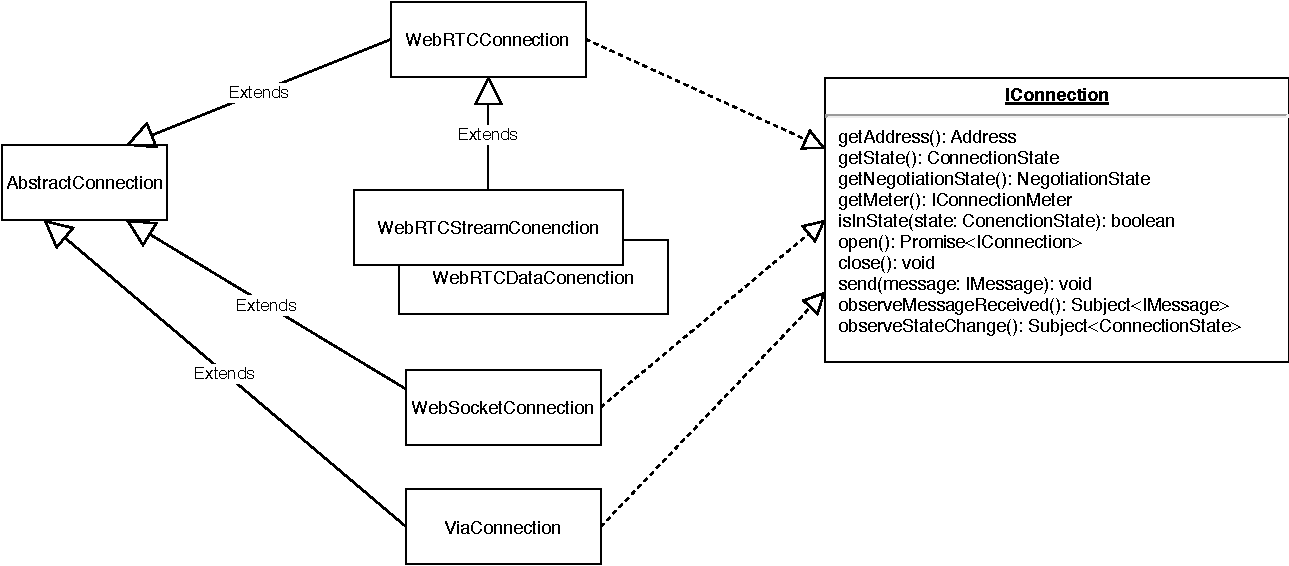
\includegraphics[width=1\textwidth]{graphics/implementation/mitosis-architecture-connections.pdf}
\caption{Connections}\label{sec:mit-connections}
\label{fig:mit-connections-uml}
\end{figure}

\vref{fig:mit-connections-uml} shows how connections are designed.

The interface specifies the methods that each connection has to implement. As some logic can be handled in a general way, an abstract connection is available. Each connection has to implement the interface but can optionally choose to extend from the abstract connection class.

Functionality that a connection has to provide is for example how to open a connection, how to send messages and so on. The WebRTC Connection has to implement for example the negotiation process that is explained in \vref{par:webrtc-con-negotiation}.

A connection itself is providing a \lstinline|ConnectionMeter| which is used by the \lstinline|RemotePeerMeter| (\vref{sec:mit-peer-meter}) to determine the connection quality.